% =====================================================================
%  Environmental Economics -- BSc AIDAMS
%  Track 7: Stranded assets
%
%  Compile with:  pdflatex track7_report.tex   (run it twice)
%  Figures expected in ./figures/ , produced by track7_stranded_assets.ipynb
%  Optional: put essec-logo.png next to this file and it appears on the
%  title page; without it the page compiles unchanged.
% =====================================================================
\documentclass[11pt,a4paper]{article}

\usepackage[utf8]{inputenc}
\usepackage[T1]{fontenc}
% Both are present on Overleaf and in any full TeX Live; guarded so the file
% also compiles on a minimal installation.
\IfFileExists{babel.sty}{\usepackage[english]{babel}}{}
\IfFileExists{lmodern.sty}{\usepackage{lmodern}}{}
\usepackage[margin=2.4cm]{geometry}
\usepackage{graphicx}
\usepackage{booktabs}
\usepackage{amsmath}
\usepackage{caption}
\usepackage{fancyhdr}
\usepackage[hidelinks]{hyperref}
\usepackage{url}

% --- page numbers bottom right ---------------------------------------
\pagestyle{fancy}
\fancyhf{}
\renewcommand{\headrulewidth}{0pt}
\fancyfoot[R]{\thepage}

% --- captions ---------------------------------------------------------
\captionsetup{font=small,labelfont=bf,justification=justified,
              singlelinecheck=false,width=\textwidth}

% --- classic indented paragraphs, no vertical gaps --------------------
\setlength{\parindent}{1.5em}
\setlength{\parskip}{0pt}
\linespread{1.03}\selectfont

% --- let floats share pages with text instead of standing alone -------
\renewcommand{\topfraction}{0.92}
\renewcommand{\bottomfraction}{0.85}
\renewcommand{\textfraction}{0.06}
\renewcommand{\floatpagefraction}{0.80}
\setcounter{topnumber}{2}
\setcounter{bottomnumber}{1}
\setcounter{totalnumber}{3}

\newcommand{\CoalAge}{29}
\newcommand{\CoalRemaining}{16}
\newcommand{\CoalModelMin}{1{,}528}
\newcommand{\CoalModelMax}{1{,}763}
\newcommand{\CoalEligible}{2{,}015}
\newcommand{\GasAge}{26}
\newcommand{\GasRemaining}{6}
\newcommand{\GasModelMin}{622}
\newcommand{\GasModelMax}{749}
\newcommand{\GasEligible}{1{,}812}
\newcommand{\ChinaAllocation}{1{,}189}
\newcommand{\IndiaAllocation}{221}
\newcommand{\USAllocation}{165}
\newcommand{\ChinaShare}{50.4}
\newcommand{\AsiaCoalShare}{91.8}
\newcommand{\MEAGasShare}{34.2}
\newcommand{\OECDGasShare}{34.6}
\newcommand{\ConstructionCoal}{260}

\begin{document}
\hypersetup{pageanchor=false}
\begin{titlepage}
\centering
\vspace*{1.0cm}
{\normalsize ESSEC Business School / CentraleSupélec\par}\vspace{0.3cm}
{\normalsize Environmental Economics\par}\vspace{0.3cm}
{\normalsize BSc AIDAMS\par}\vspace{6.0cm}
{\LARGE\bfseries Track 7 Stranded Assets\par}\vspace{1.0cm}
{\large How much fossil capacity would have to retire before the end of its technical life along different transition pathways and where is that concentrated\par}\vspace{1.0cm}
{\normalsize Authors\par}\vspace{0.3cm}
{\large Edgar Gusching\\

Adrien Labergere\\

Louis Bettelli\\

Oscar Moulet\\

Lucas Magret Delord\\

Victor Henz\par}\vspace{6.0cm}
{\large Supervised by Caterina Seghini\par}\vspace{0.3cm}
{\large October 2026\par}\vspace{0.3cm}
\end{titlepage}
\setcounter{page}{1}
\hypersetup{pageanchor=true}
\section{The question}

A power station is a long-lived investment. If electricity markets or climate policy reduce demand for its output before its assumed operating life ends, some of that investment may fail to earn the return expected when it was built. The financial consequences depend on costs, revenues and ownership; here we study the physical capacity potentially exposed to early retirement.

We ask how much of the existing coal- and gas-fired fleet, measured in gigawatts, would exceed the installed capacity allowed by different transition pathways before the end of its assumed life. We then ask where this excess is concentrated by country, technology and plant age. The answer is conditional on a scenario, an evaluation date, a lifetime assumption and a rule for allocating the excess.

This question is relevant to central banks, lenders and governments assessing transition risk. Climate-related scenarios are used in financial stability analysis {[}6{]}, while GEM's assessment of oil and gas retirement highlights the gap between existing infrastructure and climate pathways {[}4{]}. Our exercise provides a physical exposure measure rather than a monetary valuation or a forecast of actual closures.

Two choices carry much of the result. Technical lifetime is not observed directly, so we distinguish the retirement ages recorded in the data from the lifetimes we assume for the operating fleet. The plant inventory and the scenarios also have different coverage and geographical resolution. We make these differences explicit and examine how sensitive the answer is to the lifetime assumptions.

\section{Description of the data}

The analysis combines a unit-level inventory of the existing fossil fleet with a set of modelled transition pathways.

\paragraph{The plant inventory.}

Global Energy Monitor (GEM) publishes two trackers covering the world's fossil-fired power stations. The Global Coal Plant Tracker (July 2026 release) contains 14,674 coal units across 111 countries and areas, and the Global Oil and Gas Plant Tracker (August 2026 release) contains 14,099 oil and gas units across 171 countries and areas. Both are released under a CC BY 4.0 licence, were accessed on 14 October 2026, and are obtained by submitting a short form rather than by direct download. Full citations, including release dates and access dates, are given in the references. The trackers are updated approximately twice a year. Coal coverage starts at 30~MW. The oil and gas tracker generally includes units with a capacity of at least 50~MW, with a lower threshold of 20~MW in the European Union and the United Kingdom. For combined-cycle plants and groups of engines, this minimum may apply to their combined capacity rather than to each unit. Coverage of smaller units is therefore incomplete.

Each row is a generating unit rather than a station, carrying installed capacity in megawatts, country, operating status, the year the unit started generating and for closed units the year it was retired. We use the operating units, which are the capacity examined in this report, and retired units which provide observed retirement ages. Capacity under construction is excluded because it is not yet operating. The coal tracker contains 260~GW under construction, this is a separate stock, not included in our 2040 gap. Construction can already involve sunk costs, but assessing those projects is outside our fixed-fleet exercise.

Two construction choices affect the totals. The oil and gas tracker mixes gas- and oil-fired units in one sheet, and we keep those whose fuel classification is Gas, Multi Fuel or LNG only, dropping the 1,312 oil-only units. Multi-fuel units are retained because they are gas-capable; excluding them would cut our operating gas stock by about a fifth. This is a classification choice, not proof that every plant assigns multi-fuel capacity in the same way. Gas units are then grouped by turbine technology, separating combined cycle, gas turbine and steam turbine from a residual category, because realised lifetimes differ sharply between them. Coal is treated as one group, since the tracker's combustion technology field distinguishes boiler types by thermal efficiency rather than by longevity. We also chose not to use the tracker's own remaining plant lifetime column as it is a derived assumption rather than an observed figure.

\paragraph{Missing observations and the observation window.}

Start years are missing for 69 operating coal units and 137 operating gas units, around 1.3 per cent of the fleet by count and less by capacity. These are dropped from everything that depends on age. We do not impute a vintage, since an invented start year would propagate directly into the retirement date.

A more serious limitation concerns observed closures, the records used here contain retirements from 2000 onwards for coal and from 2020 onwards for gas. Plants that closed before those windows are absent entirely. The recorded retirement ages are therefore a selected sample, not the distribution of technical lifetimes for all plants ever built. There are 3,087 usable coal closures and only 280 gas closures. This makes the gas evidence particularly limited.

The notebook checks for missing or non-positive operating capacity, duplicate operating-unit identifiers, commissioning years after 2026 and unmapped countries. No operating capacities are missing in the supplied files. Missing commissioning years account for 19.2~GW and are excluded from age-dependent calculations. For the retirement-age description, observations without both dates or with an age outside 0--100 years are excluded.

\paragraph{The scenarios.}

The Network for Greening the Financial System publishes the NGFS Climate Scenarios Data Set through the IIASA Scenario Explorer. We use version 5.1, released on 20 March 2026 and accessed on 14 October 2026 under the guest login, which reports variables at five-year intervals from 2020 to 2100 for each scenario and each underlying integrated assessment model (IAM). We take three models, GCAM 6.0, MESSAGEix-GLOBIOM 2.0 and REMIND-MAgPIE 3.3-4.8, and three scenarios spanning the families presented in the course: Net Zero 2050 as an orderly transition, Delayed transition as a disorderly one, and Current Policies as a hot-house world. A fourth model variant reporting integrated physical damages is excluded because it covers only a subset of regions.

The variables are \texttt{Capacity\textbar{}Electricity\textbar{}Coal} and \texttt{Capacity\textbar{}Electricity\textbar{}Gas}, both measured in gigawatts of installed capacity. The track brief asks for fossil generation paths. We retrieve those too, using \texttt{Secondary\ Energy\textbar{}Electricity\textbar{}Coal} and its gas equivalent in EJ/year, and report their levels in the notebook. The capacity comparison uses GW on both sides. Converting generation into installed capacity would require an assumption about utilisation, potentially varying by region, technology and year. Our comparison therefore addresses installed capacity directly, the generation check in Section~4 shows why reductions in output need not imply the same reduction in capacity.

\paragraph{Matching the two sources.}

The two data sets do not share a geography, and reconciling them is where we lose the most. The inventory is country-level and the scenarios are not. The extract contains 38 region labels for GCAM and 18 each for MESSAGE and REMIND, including World and the five R5 aggregates; these are not counts of native model regions. Native region definitions differ across models. All three also report the five IPCC R5 aggregates, which are the finest geography on which the three can be compared without reconciling native regions by hand. We therefore map every country to one of the five R5 regions, using the MESSAGE eleven-region classification from the \texttt{country\_converter} package as an intermediate step and assigning by hand the small territories it can not resolve. The grouping of MESSAGE regions into R5 aggregates is not assumed: we verify for selected MESSAGE scenario-years that the native regions reproduce the R5 value the NGFS file itself reports to within 0.001~GW, and that the five regions sum to World within that tolerance in every model, scenario and comparison year used in the analysis. Every unit is matched.

What is lost is country resolution on the scenario side. We can still describe the stock country by country, and Section~4 does, but the comparison between fleet and pathway exists only across five large regions, so any country figure we report is an allocation of a regional result rather than an independent estimate.

\paragraph{The starting year.}

The inventory is a 2026 snapshot, so our committed path starts in 2026 rather than treating it as an observed 2025 fleet. NGFS capacity for 2026 is linearly interpolated between 2025 and 2030 within each model, region and scenario. The starting capacity within assumed life is 2,015~GW for coal and 1,812~GW for gas, below the full observed stock because some operating units have missing ages or already exceed the assumed lifetime. The notebook compares both stocks with each scenario's interpolated starting value. Differences in coverage and assumptions can contribute to later gaps and we do not apply an arbitrary constant subtraction to remove them.

\section{Summary statistics}

Table~1 describes the operating fleet, which is the stock that is at risk of being stranded. Table~2 splits the same capacity across the five regions used for the comparison with the scenarios.

\begin{table}[htbp]
\centering
\caption{The operating coal and gas fleet, by technology group. Capacity is installed capacity in gigawatts and ages are measured relative to 2026; units with a missing start year are excluded from the age columns. Source: Global Coal Plant Tracker (July 2026 release) and Global Oil and Gas Plant Tracker (August 2026 release), Global Energy Monitor; authors' calculations.}
\label{tab:fleet}
\small
\begin{tabular}{llrrrrrr}
\toprule
Fuel & Technology group & Units & Capacity & Mean unit & Mean age & S.d.\ age & Countries \\
 & & & (GW) & (MW) & (years) & (years) & \\
\midrule
Coal & All coal            & 6{,}591 & 2{,}226.5 & 337.8 & 22.4 & 16.6 & 74 \\
\addlinespace
Gas  & Combined cycle      & 3{,}526 & 1{,}397.4 & 396.3 & 17.2 & 10.6 & 108 \\
Gas  & Gas turbine         & 3{,}007 &   327.8 & 109.0 & 21.8 & 12.7 & 81 \\
Gas  & Steam turbine       & 1{,}861 &   339.4 & 182.4 & 36.7 & 20.8 & 62 \\
Gas  & Other or unknown    &   345 &    41.3 & 119.6 & 11.3 & 10.5 & 78 \\
\midrule
\multicolumn{2}{l}{Total} & 15{,}330 & 4{,}332.2 & 282.6 & 22.5 & 16.3 & 147 \\
\bottomrule
\end{tabular}
\end{table}

Three features of Table~1 shape everything that follows. The fleet is young: the average operating coal unit is 22 years old and the average combined-cycle gas unit only 17, so the assumed lifetime strongly affects how much capacity remains in the 2040s. The coal fleet is concentrated, appearing in 74 countries, while the gas fleet is not, present in 108 countries for combined-cycle gas alone. And the variation within gas is large, with steam turbines averaging 37 years against 17 years for combined cycle, a twenty-year gap that makes it clear gas should not be treated as a single technology.

\begin{table}[htbp]
\centering
\caption{Operating capacity by R5 region and fuel, in gigawatts. The R5 regions are the five IPCC aggregates reported by all three integrated assessment models. Source: as Table~1; authors' calculations.}
\label{tab:regions}
\small
\begin{tabular}{lrrr}
\toprule
Region & Coal (GW) & Gas (GW) & Total (GW) \\
\midrule
Asia                    & 1{,}725 &   440 & 2{,}165 \\
OECD and EU             &   373 &   941 & 1{,}314 \\
Middle East and Africa  &    56 &   436 &   491 \\
Reforming Economies     &    58 &   167 &   224 \\
Latin America           &    15 &   122 &   137 \\
\midrule
World                   & 2{,}227 & 2{,}106 & 4{,}332 \\
\bottomrule
\end{tabular}
\end{table}

The asymmetry in Table~2 is the most important descriptive fact in this paper. Asia holds 77 per cent of world coal capacity but only 21 per cent of gas capacity, while the OECD and EU hold 45 per cent of gas and 17 per cent of coal. Coal and gas are not two versions of the same problem: they sit in different places, and have different age and technology profiles.

\section{Figures}

\subsection*{Observed retirement ages and assumed lifetimes}

For closed units with usable dates, retirement age is retirement year minus commissioning year. Figure~1 and Table~3 describe these observed ages. The median recorded coal closure occurred at 39 years; the gas medians are 25 years for combined cycle, 32 for gas turbines and 49 for steam turbines. These summaries describe the recorded closures, not the eventual lifespan of the current operating fleet. We do not fit a survival model or treat these sample medians as estimated technical expiry dates.

\begin{figure}[htbp]
\centering
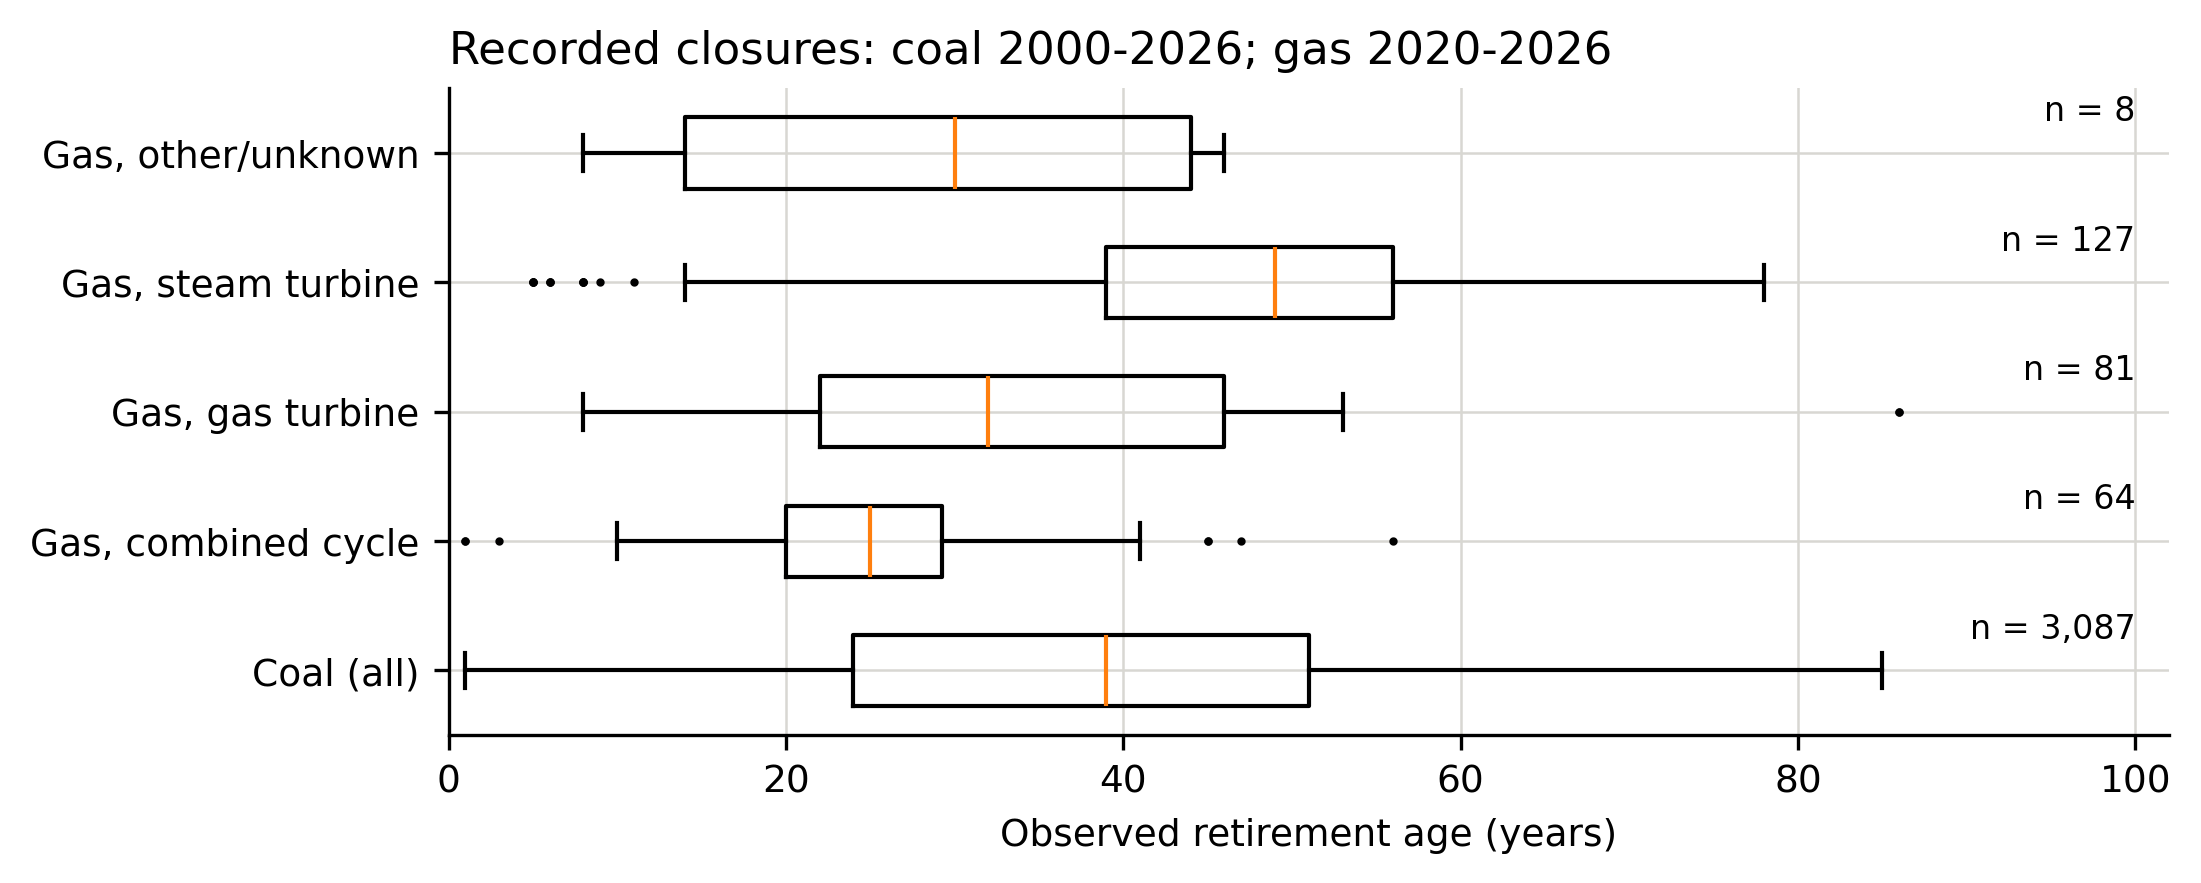
\includegraphics[width=0.88\textwidth]{figures/fig1_lifetimes.png}
\caption{Observed retirement ages of units worldwide, with coal closures recorded in 2000--2026 and gas closures in 2020--2026. Boxes show the interquartile range and median; whiskers extend to observations within 1.5 interquartile ranges, with remaining observations shown as points. Labels give sample sizes. Recorded steam turbine retirements occur at older ages than combined-cycle retirements, but the selected samples do not establish technical lifetimes. Source: GEM coal tracker, July 2026, and oil and gas tracker, August 2026; authors' calculations.}
\label{fig:lifetimes}
\end{figure}

\begin{table}[htbp]
\centering\small
\caption{Recorded retirement ages and assumed lifetimes, in years. The first four numeric columns describe recorded closures; the final column is an assumption used for operating units, not an estimated parameter. Coverage and sources as in Figure~1.}
\label{tab:lifetimes}
\begin{tabular}{lrrrrr}
\toprule
Technology & Closures & Median & 25th pct. & 75th pct. & Assumed \\
\midrule
Coal (all) & 3087 & 39.0 & 24.0 & 51.0 & 45 \\
Gas: combined cycle & 64 & 25.0 & 20.0 & 29.2 & 30 \\
Gas: gas turbine & 81 & 32.0 & 22.0 & 46.0 & 35 \\
Gas: other/unknown & 8 & 30.0 & 14.0 & 44.0 & 35 \\
Gas: steam turbine & 127 & 49.0 & 39.0 & 56.0 & 45 \\
\bottomrule
\end{tabular}

\end{table}

For coal we use 45 years, a rounded scenario assumption close to the historical global average of about 46 years discussed by Cui et al.~{[}1{]}, who also consider operation over 50 years. For gas we use 30 years for combined cycle, 35 for gas turbines and the residual group, and 45 for steam turbines. The gas assumptions are informed by the recorded ages but are not statistically identified by this short observation window. Neither their precise levels nor their ordering should be treated as a finding about the entire operating fleet.

These thresholds are deliberately exposed to sensitivity analysis. A diagnostic also shows their limitations: 208~GW of operating coal with known commissioning years has reached or exceeded 45 years, and 152~GW of gas steam turbines has reached or exceeded its assumed life, about 45 per cent of that technology's operating capacity for which age data is present. Such units are absent from our committed path from the start. The thresholds can not therefore be interpreted as physical limits, longer lifetimes would retain more of the existing fleet and can increase the calculated excess.

\subsection*{How much capacity has to close early}

We define committed capacity as the part of the 2026 operating fleet whose commissioning year is no later than the evaluation year and whose assumed natural retirement date is later. Natural retirement is commissioning year plus assumed lifetime. The path adds no new plants and applies no early closures. For each fuel, world excess capacity at date \(t\) is

\begin{equation}
{gap}_{t} = \max({committed}_{t} - {scenario}_{t},0).
\label{eq:gap}
\end{equation}

All quantities are in GW. The gap is a stock of capacity that is incompatible with the scenario at that date under our assumptions. It is not an annual retirement rate or cumulative historical retirements: previously affected units can disappear from later gaps once they reach their assumed natural retirement date.

\begin{figure}[htbp]
\centering
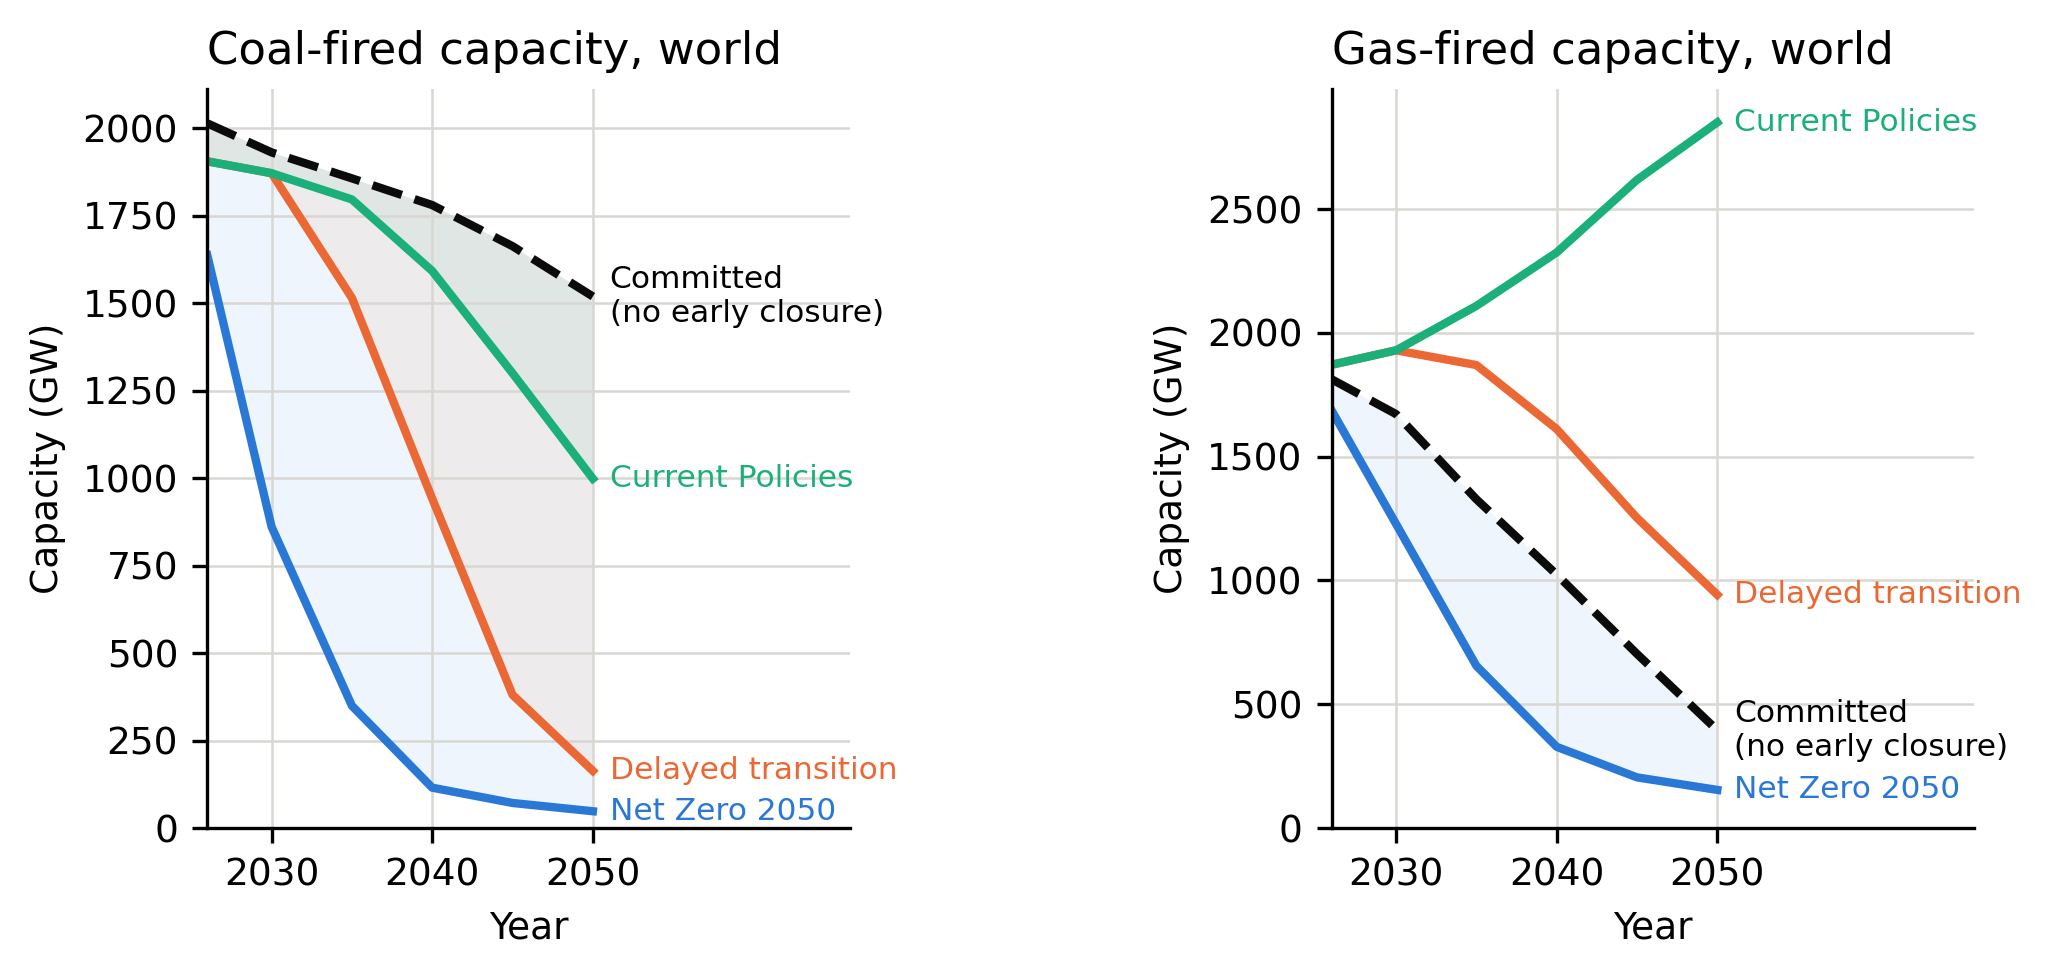
\includegraphics[width=0.80\textwidth]{figures/fig2_committed_vs_scenarios.png}
\caption{Committed capacity against three NGFS pathways, world totals, 2026 to 2050. The dashed line is the capacity still operating if every unit runs to the end of its assumed technical life, which is 45 years for coal and 30 to 45 years by technology for gas. Coloured lines are the mean across the three integrated assessment models, and shading shows positive differences. The initial 2026 scenario values are interpolated between 2025 and 2030. The coal gap is much larger under Net Zero 2050 in 2030; positive gaps also occur under the other scenarios before 2035. At the base lifetime assumptions, the world gas gap appears only under Net Zero 2050. Source: Global Energy Monitor trackers (July and August 2026 releases); NGFS Climate Scenarios Data Set v5.1 (March 2026 release); authors' calculations.}
\label{fig:committed}
\end{figure}

Figure~2 gives the central result. In 2040 under Net Zero 2050, the world excess is 1,665~GW of coal and 696~GW of gas. The coal gap falls to 1,471~GW by 2050 because more units reach their assumed end of life. Under Delayed transition, the coal gap rises from about 60~GW in 2030 to 839~GW in 2040 and 1,356~GW in 2050. Current Policies gives a smaller but still substantial coal gap of 521~GW in 2050. At the base lifetimes, world gas capacity within assumed life does not exceed the mean capacity pathway under Current Policies or Delayed transition, this does not establish that every existing gas unit is retained.

For the detailed 2040 Net Zero 2050 allocation, we apply equation~(1) separately within each R5 region and fuel. Within each region we allocate the gap to the oldest units first, breaking ties by unit identifier. We allocate only the required capacity of the final unit, so each regional total matches exactly. This fraction is an accounting device, not a claim that a plant can be partly retired. Regional gaps can generally sum to more than the world gap because a surplus in one region can not offset a shortage elsewhere. For this specific case their sums agree with the world gaps. Country results below are allocations of those regional totals, not independent country forecasts.

\begin{figure}[htbp]
\centering
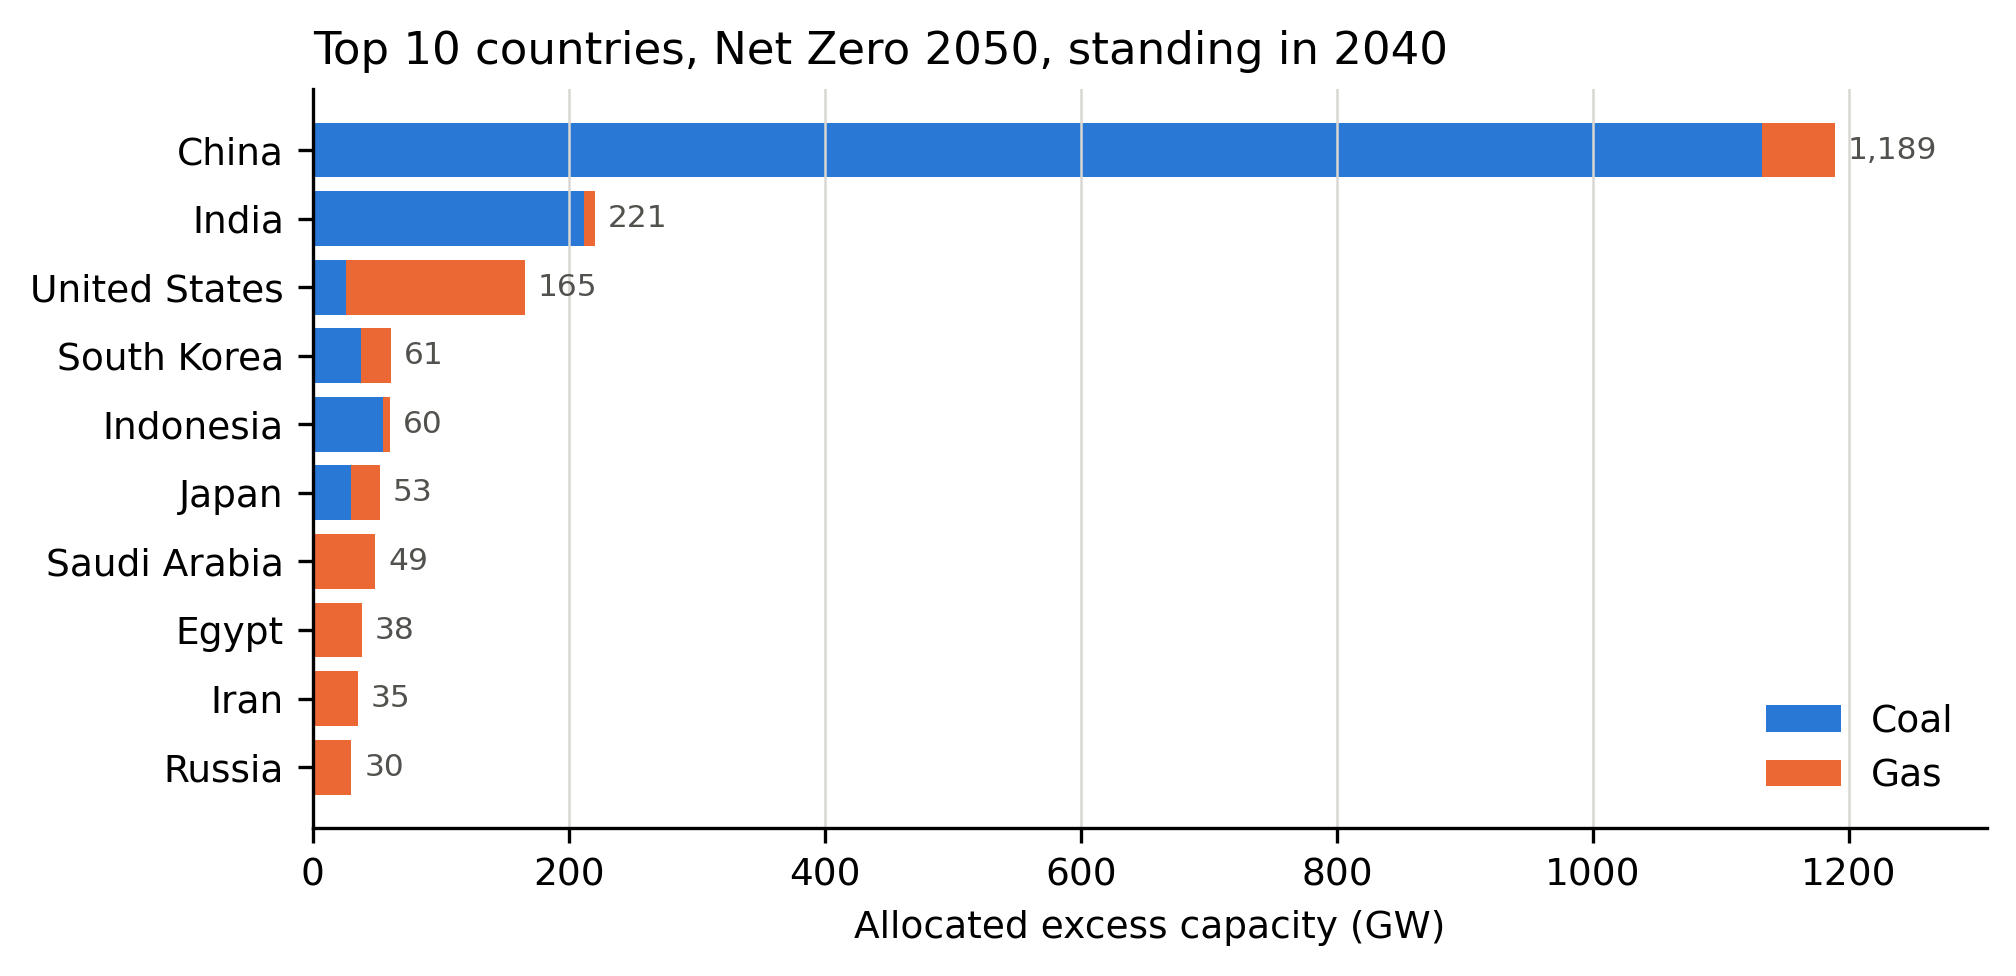
\includegraphics[width=0.80\textwidth]{figures/fig4_country_profile.png}
\caption{Allocated excess capacity by country in 2040 under Net Zero 2050, using the mean of three IAMs. Allocations fill each R5 region's fuel-specific gap, oldest first, with unit-ID tie-breaking and a fractional boundary unit. China receives 1,189~GW, India 221~GW and the United States 165~GW. The concentration is conditional on the allocation rule and lifetime assumptions. Source: GEM trackers, July/August 2026; NGFS v5.1, March 2026; authors' calculations.}
\label{fig:country}
\end{figure}

In this allocation, Asia accounts for 91.8 per cent of coal excess, and China accounts for 50.4 per cent of the combined coal and gas total. Gas is more dispersed: the Middle East and Africa account for 34.2 per cent and the OECD and EU for 34.6 per cent. These results identify where physical exposure is concentrated under the stated convention. They do not identify which owners bear financial losses.

Table~4 adds the technology dimension. Gas capacity is grouped by turbine type, while coal is pooled because it uses one assumed lifetime. The notebook also provides the more detailed coal combustion-technology breakdown.

\begin{table}[htbp]
\centering\small
\caption{Allocated excess capacity by technology, Net Zero 2050 in 2040. Shares are within each fuel. This is the regional oldest-first allocation used in Figure~3, not a technology-specific scenario projection. Source: GEM trackers, July/August 2026; NGFS v5.1; authors' calculations.}
\label{tab:technology}
\begin{tabular}{llrr}
\toprule
Fuel & Technology & Allocated GW & Share within fuel (\%) \\
\midrule
Coal & Coal (all) & 1,665.2 & 100.0 \\
Gas & Gas: combined cycle & 476.8 & 68.5 \\
Gas & Gas: gas turbine & 131.2 & 18.9 \\
Gas & Gas: other/unknown & 21.2 & 3.0 \\
Gas & Gas: steam turbine & 66.4 & 9.5 \\
\bottomrule
\end{tabular}

\end{table}

\begin{figure}[htbp]
\centering
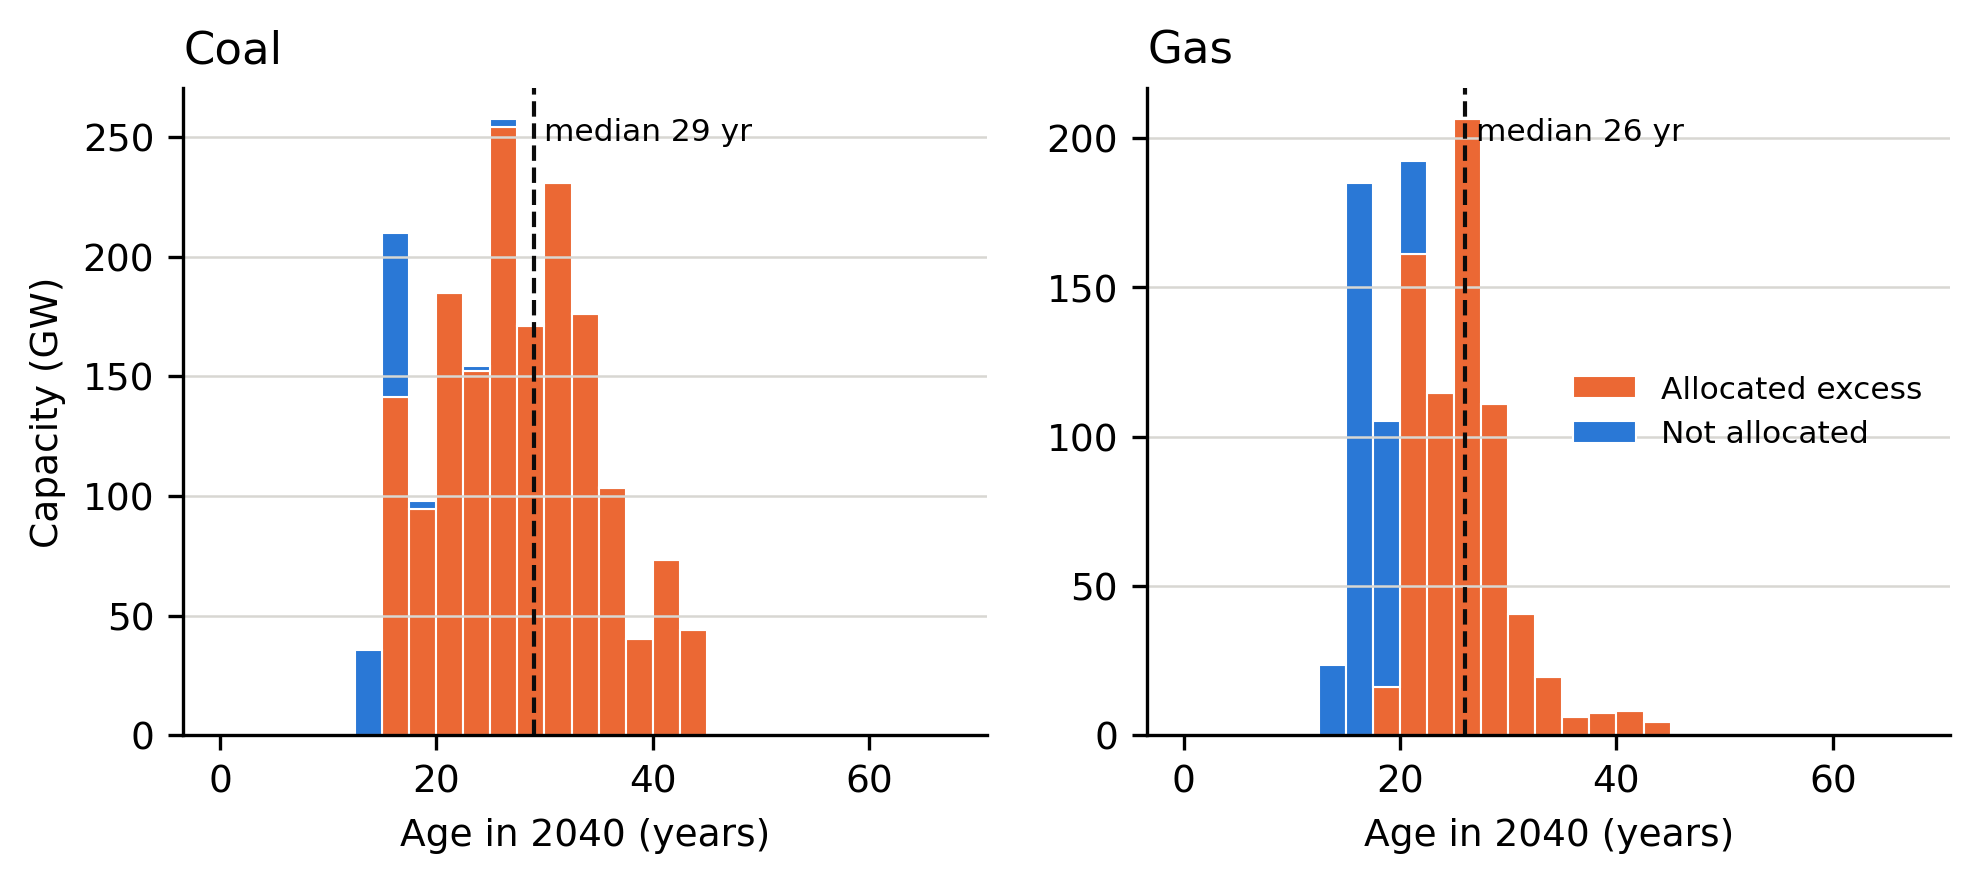
\includegraphics[width=0.80\textwidth]{figures/fig5_age_profile.png}
\caption{Age in 2040 of the committed fleet, split into allocated excess and unallocated capacity under Net Zero 2050. The median age among units with positive allocation is 29 years for coal and 26 for gas. Medians count units, including the fractionally allocated boundary units, rather than weighting by MW. These are evaluation-date ages, not estimated closure ages. Source: GEM trackers, July/August 2026; NGFS v5.1; authors' calculations.}
\label{fig:age}
\end{figure}

Figure~4 shows that allocated excess is not confined to units close to the assumed end of life. Among units with positive allocation, median remaining assumed life in 2040 is 16 years for coal and 6 for gas. We do not assign an actual closure year. Closing before 2040 would mean a younger closure age and more years of life foregone than this target-date measure. The unallocated portion also does not necessarily run to its natural end of life: it is simply not needed to fill this particular regional gap. Monetary losses can not be inferred from remaining years alone.

\subsection*{How much the lifetime assumption matters}

\begin{figure}[htbp]
\centering
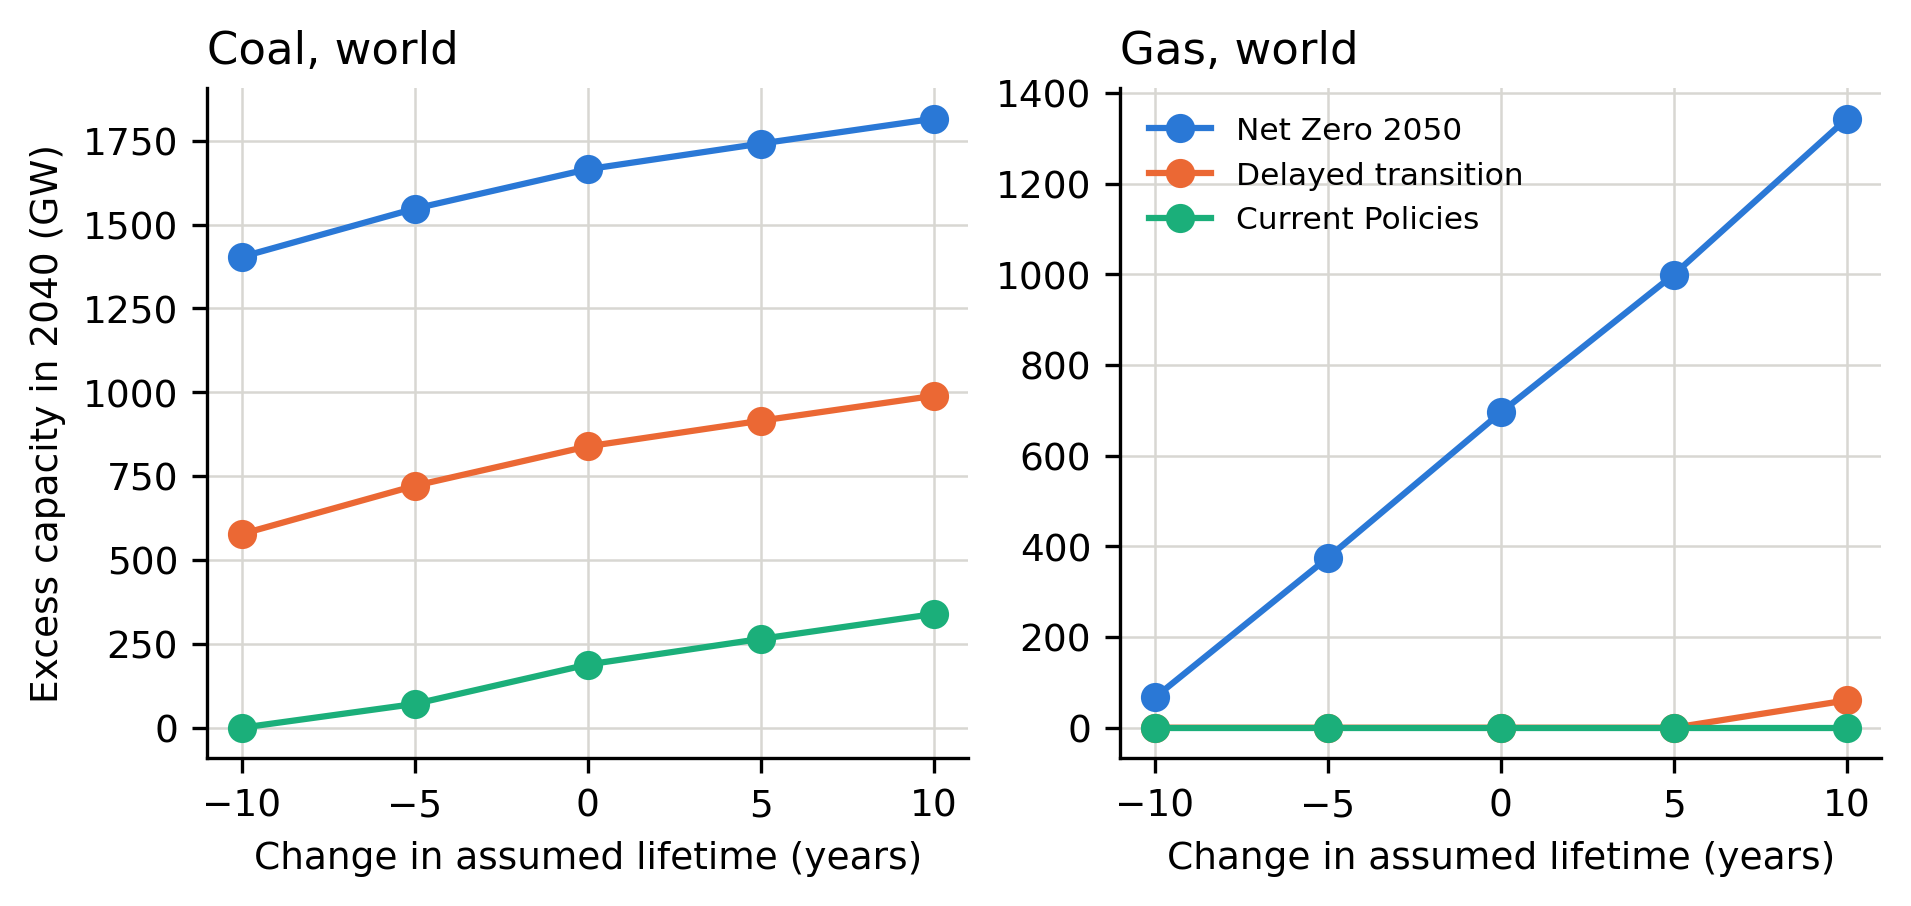
\includegraphics[width=0.80\textwidth]{figures/fig6_sensitivity.png}
\caption{World excess capacity in 2040, against the assumed technical lifetime. All technology-specific lifetimes are shifted together by the amount on the horizontal axis, so zero is the base case of 45 years for coal and 30 to 45 years for gas. Coal is robust, with the Net Zero 2050 figure moving from 1,404 to 1,816~GW across a twenty-year swing, a range of less than 30 per cent. Gas is not, since the same swing moves it from 67 to 1,344~GW, a factor of twenty. Source: Global Energy Monitor trackers (July and August 2026 releases); NGFS v5.1 (March 2026 release); authors' calculations.}
\label{fig:sensitivity}
\end{figure}

The brief asks how far the answer moves if the lifetime assumption changes, and Figure~5 give shows it depends entirely on which fuel is being asked about.

For coal, shifting the assumed lifetime from 35 to 55 years moves the 2040 Net Zero 2050 world gap from 1,404 to 1,816~GW. Every value tested leaves an excess above one thousand GW. For gas, shifting all technology lifetimes by the same amounts moves the gap from 67 to 1,344~GW. The precise gas total is therefore much more sensitive to these assumptions. The range is a scenario sensitivity, not a statistical confidence interval.

Separately, retaining the base lifetimes and comparing individual models gives a 2040 Net Zero coal gap of 1,528--1,763~GW and a gas gap of 622--749~GW. Both model choice and lifetime matter. These checks concern totals, they do not establish that every country share, technology share or age statistic remains unchanged under alternative assumptions.

\subsection*{Robustness: capacity against generation}

The notebook reports generation paths in EJ/year and compares generation and capacity indices with 2025 set to 100. By 2050 under Delayed transition, coal generation is about 3 per cent of its 2025 level versus 9 per cent for capacity; the corresponding gas indices are 35 and 51. Under Current Policies, coal indices are 60 for generation and 52 for capacity. The relative movement varies by fuel, date and scenario: for example, delayed-transition gas in 2040 has generation index 88 and capacity index 87.

These differences are consistent with changes in utilisation. Lower generation does not require a proportionate closure of installed capacity, so the indexed comparison can not prove that a generation-based calculation would give a larger retirement estimate. We use capacity to answer the physical-capacity question directly and retain utilisation as a limitation. Similarly, differences between the 2026 plant inventory and interpolated scenario levels are not resolved by subtracting a single baseline discrepancy from all future years.

\section{Econometrics}

We estimate observed retirement age by ordinary least squares (OLS), using 1,129 closures in 2020--2026: 849 coal and 280 gas units in 61 countries or areas. Both models use the same sample with usable dates and positive capacity. Model 1 includes technology indicators; Model 2 adds size, R5-region indicators and retirement-year indicators:

\begin{equation}
A_{i} = \alpha + \sum_{k \neq coal}^{}\beta_{k}D_{ik} + \gamma\log_{2}C_{i} + \delta_{r(i)} + \lambda_{y(i)} + \varepsilon_{i}.
\label{eq:retirement}
\end{equation}

Here A is retirement age in years, D denotes technology indicators with coal as the reference, C is capacity in MW, and the region and year indicators absorb differences between these groups. Model 1 omits the size, region and year terms. A technology coefficient is an adjusted difference from coal in years, the size coefficient is the difference associated with doubling capacity.

\begin{table}[htbp]
\centering\small
\caption{OLS coefficients in years, with HC3 standard errors in parentheses. Technology rows show differences from coal: negative values indicate younger retirement. The capacity row shows the difference associated with doubling MW. Intercept, region and year coefficients are omitted. Source: GEM trackers, July/August 2026; authors\textquotesingle{} calculations.}
\label{tab:econometrics}
\begin{tabular}{lrr}
\toprule
Coefficient & Technology only & With controls \\
\midrule
Gas, combined cycle (vs coal) & -14.49 (1.43) & -14.80 (1.76) \\
Gas, gas turbine (vs coal) & -5.29 (1.84) & -12.42 (1.92) \\
Gas, steam turbine (vs coal) & 5.54 (1.60) & -1.60 (1.69) \\
Gas, other/unknown (vs coal) & -10.58 (6.69) & -14.01 (5.02) \\
Capacity doubling & -- & -0.67 (0.38) \\
\midrule
Region and year indicators & No & Yes \\
Closures & 1129 & 1129 \\
R-squared & 0.061 & 0.368 \\
\bottomrule
\end{tabular}

\end{table}

With controls, combined-cycle gas units retired 14.80 years younger than coal (95 per cent HC3 interval: 11.34--18.26 years younger), and gas turbines 12.42 years younger (8.65--16.19). Steam turbines show no clear difference from coal. Doubling capacity is associated with a 0.67-year lower retirement age, but its interval, \ensuremath{-}1.42 to 0.08 years, includes zero. Country-clustered standard errors across 61 clusters preserve these main conclusions; the notebook reports both uncertainty calculations.

These are conditional correlations among recorded closures, not causal effects or estimates of technical expiry dates. The common observation window does not remove selection into retirement or differences in tracker coverage. The residual technology group has only eight observations. We therefore retain the explicit lifetime assumptions and sensitivity analysis rather than replacing them with fitted retirement ages.

\section{What we can and can not conclude}

Under our base lifetime assumptions, 1,665 GW of coal capacity and 696 GW of gas capacity from the 2026 operating fleet exceed the Net Zero 2050 capacity pathway in 2040. This is about 2,361 GW of capacity that would otherwise remain within its assumed operating life. The pathway matters: the corresponding 2040 coal gap is 839 GW under Delayed transition and 188 GW under Current Policies. At the base assumptions, neither of these two scenarios produces a positive world gas gap in 2040.

The 2040 Net Zero allocation places 91.8 per cent of coal exposure in Asia. China receives 1,189 GW of combined coal and gas allocation, followed by India with 221 GW and the United States with 165 GW. China alone accounts for 50.4 per cent of the combined total. Within gas, combined-cycle units account for 477 GW, or 68.5 per cent of the gas allocation. Coal is pooled into one lifetime group; the gas results show why the technology distinction matters.

The allocated capacity is not limited to units approaching their assumed retirement dates. In 2040, the median age among units receiving a positive allocation is 29 years for coal and 26 years for gas, with median remaining assumed lives of 16 and 6 years respectively. These are unit-count medians at the evaluation date. They show that meeting the scenario capacity level can require removing capacity with substantial assumed life remaining but they do not assign actual closure dates.

The regression also finds younger recorded retirement ages for combined-cycle gas and gas turbines than for coal after controls, but no clear size association.

The scale of coal exposure is more stable than the gas estimate. Shifting all lifetimes by ten years in either direction leaves the 2040 Net Zero coal gap between 1,404 and 1,816 GW, while the gas gap ranges from 67 to 1,344 GW. Thus the conclusion that a large coal adjustment is needed survives every lifetime assumption tested. The precise gas total depends much more heavily on the chosen lifetimes, which the short and selected retirement record can not establish reliably.

Our capacity comparison is a descriptive, conditional accounting exercise using published scenarios and an assumed natural retirement path. The gaps are capacity stocks at a date, not cumulative closures, financial losses or causal effects of policy. Country and technology allocations depend on the regional oldest-first rule, actual closure choices also depend on costs, regulation and reliability. We use scenario capacity directly and examine generation separately, so utilisation changes remain outside the retirement calculation. New construction and retrofits are outside our fixed-fleet path, and units already beyond their assumed life are excluded. Within these limits, our answer to Track 7 is that natural retirements alone leave a large coal capacity excess under Net Zero 2050, concentrated in Asia in our allocation, while the amount of gas capacity exposed is substantially less certain.

\clearpage
\begin{thebibliography}{9}
\small

\bibitem{cui2019}
Cui, R. Y., Hultman, N., Edwards, M. R., He, L., Sen, A., Surana, K., et al. (2019). Quantifying operational lifetimes for coal power plants under the Paris goals. \emph{Nature Communications}, 10, 4759. \url{https://doi.org/10.1038/s41467-019-12618-3}

\bibitem{gemcoal}
Global Energy Monitor (2026). \emph{Global Coal Plant Tracker}, July 2026 release. Accessed 14 October 2026. \url{https://globalenergymonitor.org/projects/global-coal-plant-tracker/}

\bibitem{gemgas}
Global Energy Monitor (2026). \emph{Global Oil and Gas Plant Tracker}, August 2026 release. Accessed 14 October 2026. \url{https://globalenergymonitor.org/projects/global-oil-gas-plant-tracker/}

\bibitem{gemretire}
Global Energy Monitor (2024). \emph{Oil and gas plants need to be retired five times faster to meet long-term climate goals}. February 2024. \url{https://globalenergymonitor.org/wp-content/uploads/2024/02/GEM_Global-oil-gas-plants-February-2024.pdf}

\bibitem{ngfs}
Richters, O., Kriegler, E., Bertram, C., Cui, R., Edmonds, J., Fawcett, A., et al. (2026). \emph{NGFS Climate Scenarios Data Set}, version 5.1 {[}Data set{]}. Zenodo. Released 20 March 2026, accessed 14 October 2026. \url{https://doi.org/10.5281/zenodo.17901363}

\bibitem{acpr}
Allen, T., Dees, S., Boissinot, J., Caicedo Graciano, C. M., Chouard, V., Clerc, L., et al. (2020). \emph{Climate-Related Scenarios for Financial Stability Assessment: An Application to France}. Banque de France Working Paper No.~774.

\end{thebibliography}

\section*{Statement on the use of AI}
\small

We used Claude (Anthropic) to assist with Python and LaTeX code, literature checking and drafting. We used OpenAI Codex to review consistency between the notebook and report, set up the Python environment, revise the calculations and explanations, and regenerate figures and tables. This assistance included reviewing the lifetime approach and revising the regional allocation and interpretation of plant ages. The notebook provides the calculations behind the results; we remain responsible for the analysis and the submitted work.

\end{document}
